\documentclass{extbook}[14pt]
\usepackage{multicol, enumerate, enumitem, hyperref, color, soul, setspace, parskip, fancyhdr, amssymb, amsthm, amsmath, latexsym, units, mathtools}
\everymath{\displaystyle}
\usepackage[headsep=0.5cm,headheight=0cm, left=1 in,right= 1 in,top= 1 in,bottom= 1 in]{geometry}
\usepackage{dashrule}  % Package to use the command below to create lines between items
\newcommand{\litem}[1]{\item #1

\rule{\textwidth}{0.4pt}}
\pagestyle{fancy}
\lhead{}
\chead{Answer Key for Progress Quiz 9 Version B}
\rhead{}
\lfoot{9541-5764}
\cfoot{}
\rfoot{Summer C 2021}
\begin{document}
\textbf{This key should allow you to understand why you choose the option you did (beyond just getting a question right or wrong). \href{https://xronos.clas.ufl.edu/mac1105spring2020/courseDescriptionAndMisc/Exams/LearningFromResults}{More instructions on how to use this key can be found here}.}

\textbf{If you have a suggestion to make the keys better, \href{https://forms.gle/CZkbZmPbC9XALEE88}{please fill out the short survey here}.}

\textit{Note: This key is auto-generated and may contain issues and/or errors. The keys are reviewed after each exam to ensure grading is done accurately. If there are issues (like duplicate options), they are noted in the offline gradebook. The keys are a work-in-progress to give students as many resources to improve as possible.}

\rule{\textwidth}{0.4pt}

\begin{enumerate}\litem{
Construct the lowest-degree polynomial given the zeros below. Then, choose the intervals that contain the coefficients of the polynomial in the form $ax^3+bx^2+cx+d$.
\[ \frac{5}{2}, \frac{-1}{2}, \text{ and } -7 \]The solution is \( 4x^{3} +20 x^{2} -61 x -35 \), which is option B.\begin{enumerate}[label=\Alph*.]
\item \( a \in [2, 10], b \in [36.1, 42.5], c \in [86, 95], \text{ and } d \in [30, 40] \)

$4x^{3} +40 x^{2} +89 x + 35$, which corresponds to multiplying out $(2x + 5)(2x + 1)(x + 7)$.
\item \( a \in [2, 10], b \in [18.8, 21.8], c \in [-65, -58], \text{ and } d \in [-35, -32] \)

* $4x^{3} +20 x^{2} -61 x -35$, which is the correct option.
\item \( a \in [2, 10], b \in [35.9, 37.2], c \in [42, 60], \text{ and } d \in [-35, -32] \)

$4x^{3} +36 x^{2} +51 x -35$, which corresponds to multiplying out $(2x + 5)(2x -1)(x + 7)$.
\item \( a \in [2, 10], b \in [-22.7, -19.9], c \in [-65, -58], \text{ and } d \in [30, 40] \)

$4x^{3} -20 x^{2} -61 x + 35$, which corresponds to multiplying out $(2x + 5)(2x -1)(x -7)$.
\item \( a \in [2, 10], b \in [18.8, 21.8], c \in [-65, -58], \text{ and } d \in [30, 40] \)

$4x^{3} +20 x^{2} -61 x + 35$, which corresponds to multiplying everything correctly except the constant term.
\end{enumerate}

\textbf{General Comment:} To construct the lowest-degree polynomial, you want to multiply out $(2x -5)(2x + 1)(x + 7)$
}
\litem{
Describe the end behavior of the polynomial below.
\[ f(x) = -6(x - 6)^{3}(x + 6)^{6}(x + 2)^{3}(x - 2)^{3} \]The solution is the graph below, which is option A.
    \begin{center}
        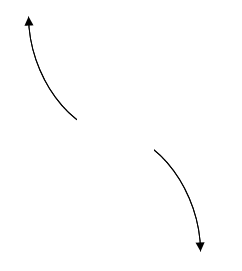
\includegraphics[width=0.3\textwidth]{../Figures/polyEndBehaviorCopyAB.png}
    \end{center}\begin{enumerate}[label=\Alph*.]
\begin{multicols}{2}
\item 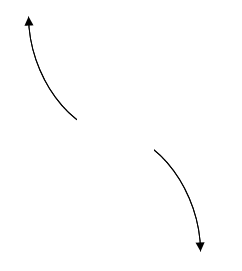
\includegraphics[width = 0.3\textwidth]{../Figures/polyEndBehaviorCopyAB.png}
\item 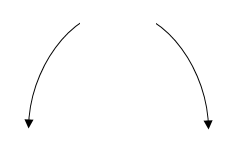
\includegraphics[width = 0.3\textwidth]{../Figures/polyEndBehaviorCopyBB.png}
\item 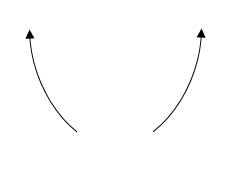
\includegraphics[width = 0.3\textwidth]{../Figures/polyEndBehaviorCopyCB.png}
\item 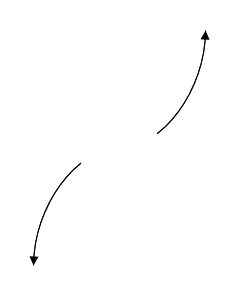
\includegraphics[width = 0.3\textwidth]{../Figures/polyEndBehaviorCopyDB.png}
\end{multicols}\item None of the above.\end{enumerate}
\textbf{General Comment:} Remember that end behavior is determined by the leading coefficient AND whether the \textbf{sum} of the multiplicities is positive or negative.
}
\litem{
Construct the lowest-degree polynomial given the zeros below. Then, choose the intervals that contain the coefficients of the polynomial in the form $x^3+bx^2+cx+d$.
\[ 4 - 3 i \text{ and } 2 \]The solution is \( x^{3} -10 x^{2} +41 x -50 \), which is option A.\begin{enumerate}[label=\Alph*.]
\item \( b \in [-15, -8], c \in [35, 44], \text{ and } d \in [-50, -44] \)

* $x^{3} -10 x^{2} +41 x -50$, which is the correct option.
\item \( b \in [-5, 4], c \in [1, 7], \text{ and } d \in [-8, 2] \)

$x^{3} + x^{2} +x -6$, which corresponds to multiplying out $(x + 3)(x -2)$.
\item \( b \in [10, 15], c \in [35, 44], \text{ and } d \in [50, 56] \)

$x^{3} +10 x^{2} +41 x + 50$, which corresponds to multiplying out $(x-(4 - 3 i))(x-(4 + 3 i))(x + 2)$.
\item \( b \in [-5, 4], c \in [-9, 0], \text{ and } d \in [6, 11] \)

$x^{3} + x^{2} -6 x + 8$, which corresponds to multiplying out $(x -4)(x -2)$.
\item \( \text{None of the above.} \)

This corresponds to making an unanticipated error or not understanding how to use nonreal complex numbers to create the lowest-degree polynomial. If you chose this and are not sure what you did wrong, please contact the coordinator for help.
\end{enumerate}

\textbf{General Comment:} Remember that the conjugate of $a+bi$ is $a-bi$. Since these zeros always come in pairs, we need to multiply out $(x-(4 - 3 i))(x-(4 + 3 i))(x-(2))$.
}
\litem{
Which of the following equations \textit{could} be of the graph presented below?

\begin{center}
    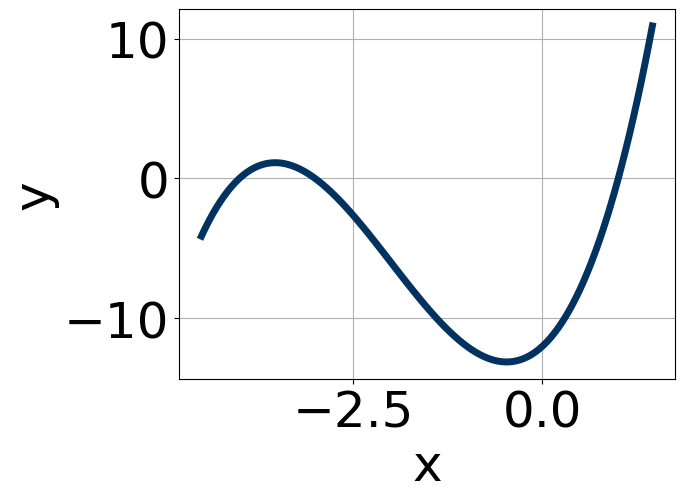
\includegraphics[width=0.5\textwidth]{../Figures/polyGraphToFunctionCopyB.png}
\end{center}


The solution is \( 3(x - 1)^{7} (x + 3)^{9} (x + 4)^{9} \), which is option D.\begin{enumerate}[label=\Alph*.]
\item \( 15(x - 1)^{4} (x + 3)^{4} (x + 4)^{9} \)

The factors $1$ and $-3$ have have been odd power.
\item \( -12(x - 1)^{10} (x + 3)^{11} (x + 4)^{11} \)

The factor $(x - 1)$ should have an odd power and the leading coefficient should be the opposite sign.
\item \( -11(x - 1)^{11} (x + 3)^{7} (x + 4)^{7} \)

This corresponds to the leading coefficient being the opposite value than it should be.
\item \( 3(x - 1)^{7} (x + 3)^{9} (x + 4)^{9} \)

* This is the correct option.
\item \( 20(x - 1)^{8} (x + 3)^{5} (x + 4)^{9} \)

The factor $1$ should have been an odd power.
\end{enumerate}

\textbf{General Comment:} General Comments: Draw the x-axis to determine which zeros are touching (and so have even multiplicity) or cross (and have odd multiplicity).
}
\litem{
Describe the zero behavior of the zero $x = 4$ of the polynomial below.
\[ f(x) = -6(x - 4)^{2}(x + 4)^{3}(x - 8)^{2}(x + 8)^{5} \]The solution is the graph below, which is option B.
    \begin{center}
        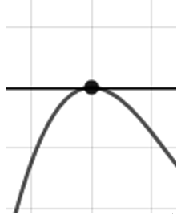
\includegraphics[width=0.3\textwidth]{../Figures/polyZeroBehaviorCopyBB.png}
    \end{center}\begin{enumerate}[label=\Alph*.]
\begin{multicols}{2}
\item 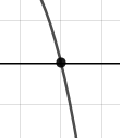
\includegraphics[width = 0.3\textwidth]{../Figures/polyZeroBehaviorCopyAB.png}
\item 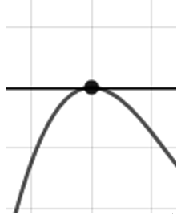
\includegraphics[width = 0.3\textwidth]{../Figures/polyZeroBehaviorCopyBB.png}
\item 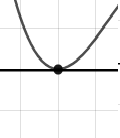
\includegraphics[width = 0.3\textwidth]{../Figures/polyZeroBehaviorCopyCB.png}
\item 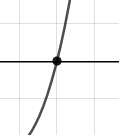
\includegraphics[width = 0.3\textwidth]{../Figures/polyZeroBehaviorCopyDB.png}
\end{multicols}\item None of the above.\end{enumerate}
\textbf{General Comment:} You will need to sketch the entire graph, then zoom in on the zero the question asks about.
}
\litem{
Describe the zero behavior of the zero $x = 5$ of the polynomial below.
\[ f(x) = -5(x + 5)^{3}(x - 5)^{4}(x + 7)^{2}(x - 7)^{4} \]The solution is the graph below, which is option B.
    \begin{center}
        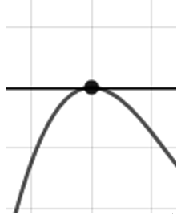
\includegraphics[width=0.3\textwidth]{../Figures/polyZeroBehaviorBB.png}
    \end{center}\begin{enumerate}[label=\Alph*.]
\begin{multicols}{2}
\item 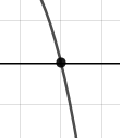
\includegraphics[width = 0.3\textwidth]{../Figures/polyZeroBehaviorAB.png}
\item 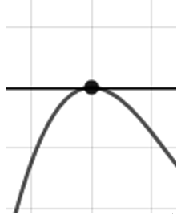
\includegraphics[width = 0.3\textwidth]{../Figures/polyZeroBehaviorBB.png}
\item 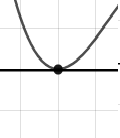
\includegraphics[width = 0.3\textwidth]{../Figures/polyZeroBehaviorCB.png}
\item 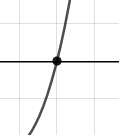
\includegraphics[width = 0.3\textwidth]{../Figures/polyZeroBehaviorDB.png}
\end{multicols}\item None of the above.\end{enumerate}
\textbf{General Comment:} You will need to sketch the entire graph, then zoom in on the zero the question asks about.
}
\litem{
Describe the end behavior of the polynomial below.
\[ f(x) = 6(x - 6)^{4}(x + 6)^{7}(x - 5)^{3}(x + 5)^{4} \]The solution is the graph below, which is option C.
    \begin{center}
        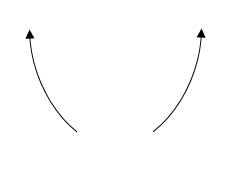
\includegraphics[width=0.3\textwidth]{../Figures/polyEndBehaviorCB.png}
    \end{center}\begin{enumerate}[label=\Alph*.]
\begin{multicols}{2}
\item 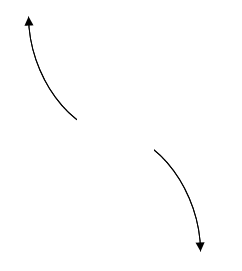
\includegraphics[width = 0.3\textwidth]{../Figures/polyEndBehaviorAB.png}
\item 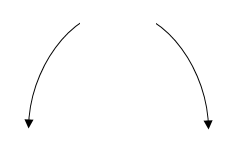
\includegraphics[width = 0.3\textwidth]{../Figures/polyEndBehaviorBB.png}
\item 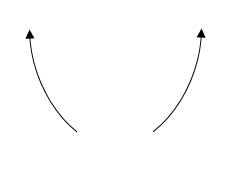
\includegraphics[width = 0.3\textwidth]{../Figures/polyEndBehaviorCB.png}
\item 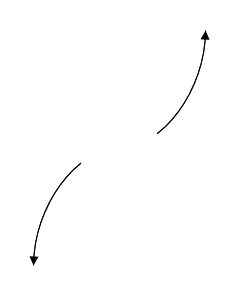
\includegraphics[width = 0.3\textwidth]{../Figures/polyEndBehaviorDB.png}
\end{multicols}\item None of the above.\end{enumerate}
\textbf{General Comment:} Remember that end behavior is determined by the leading coefficient AND whether the \textbf{sum} of the multiplicities is positive or negative.
}
\litem{
Construct the lowest-degree polynomial given the zeros below. Then, choose the intervals that contain the coefficients of the polynomial in the form $x^3+bx^2+cx+d$.
\[ -3 - 4 i \text{ and } 1 \]The solution is \( x^{3} +5 x^{2} +19 x -25 \), which is option D.\begin{enumerate}[label=\Alph*.]
\item \( b \in [-2.7, 4.7], c \in [0.81, 2.83], \text{ and } d \in [-3.5, -2.56] \)

$x^{3} + x^{2} +2 x -3$, which corresponds to multiplying out $(x + 3)(x -1)$.
\item \( b \in [-7.9, -3.5], c \in [17.28, 19.46], \text{ and } d \in [24.68, 25.62] \)

$x^{3} -5 x^{2} +19 x + 25$, which corresponds to multiplying out $(x-(-3 - 4 i))(x-(-3 + 4 i))(x + 1)$.
\item \( b \in [-2.7, 4.7], c \in [2.24, 5.06], \text{ and } d \in [-4.56, -3.05] \)

$x^{3} + x^{2} +3 x -4$, which corresponds to multiplying out $(x + 4)(x -1)$.
\item \( b \in [3.6, 7.4], c \in [17.28, 19.46], \text{ and } d \in [-25.02, -24.7] \)

* $x^{3} +5 x^{2} +19 x -25$, which is the correct option.
\item \( \text{None of the above.} \)

This corresponds to making an unanticipated error or not understanding how to use nonreal complex numbers to create the lowest-degree polynomial. If you chose this and are not sure what you did wrong, please contact the coordinator for help.
\end{enumerate}

\textbf{General Comment:} Remember that the conjugate of $a+bi$ is $a-bi$. Since these zeros always come in pairs, we need to multiply out $(x-(-3 - 4 i))(x-(-3 + 4 i))(x-(1))$.
}
\litem{
Construct the lowest-degree polynomial given the zeros below. Then, choose the intervals that contain the coefficients of the polynomial in the form $ax^3+bx^2+cx+d$.
\[ \frac{-2}{3}, \frac{1}{3}, \text{ and } \frac{5}{4} \]The solution is \( 36x^{3} -33 x^{2} -23 x + 10 \), which is option B.\begin{enumerate}[label=\Alph*.]
\item \( a \in [35, 37], b \in [-38, -31], c \in [-31, -22], \text{ and } d \in [-13, -7] \)

$36x^{3} -33 x^{2} -23 x -10$, which corresponds to multiplying everything correctly except the constant term.
\item \( a \in [35, 37], b \in [-38, -31], c \in [-31, -22], \text{ and } d \in [8, 17] \)

* $36x^{3} -33 x^{2} -23 x + 10$, which is the correct option.
\item \( a \in [35, 37], b \in [-60, -55], c \in [4, 16], \text{ and } d \in [8, 17] \)

$36x^{3} -57 x^{2} +7 x + 10$, which corresponds to multiplying out $(3x -2)(3x + 1)(4x -5)$.
\item \( a \in [35, 37], b \in [-86, -76], c \in [53, 57], \text{ and } d \in [-13, -7] \)

$36x^{3} -81 x^{2} +53 x -10$, which corresponds to multiplying out $(3x -2)(3x -1)(4x -5)$.
\item \( a \in [35, 37], b \in [32, 39], c \in [-31, -22], \text{ and } d \in [-13, -7] \)

$36x^{3} +33 x^{2} -23 x -10$, which corresponds to multiplying out $(3x -2)(3x + 1)(4x + 5)$.
\end{enumerate}

\textbf{General Comment:} To construct the lowest-degree polynomial, you want to multiply out $(3x + 2)(3x -1)(4x -5)$
}
\litem{
Which of the following equations \textit{could} be of the graph presented below?

\begin{center}
    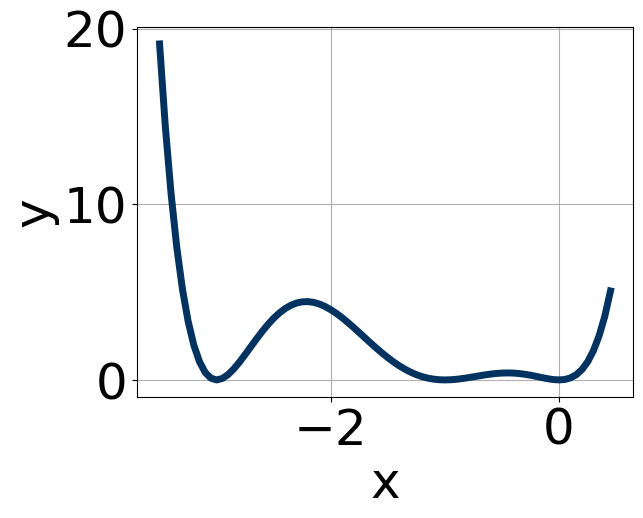
\includegraphics[width=0.5\textwidth]{../Figures/polyGraphToFunctionB.png}
\end{center}


The solution is \( 4x^{10} (x + 3)^{10} (x + 1)^{6} \), which is option A.\begin{enumerate}[label=\Alph*.]
\item \( 4x^{10} (x + 3)^{10} (x + 1)^{6} \)

* This is the correct option.
\item \( 10x^{8} (x + 3)^{8} (x + 1)^{11} \)

The factor $(x + 1)$ should have an even power.
\item \( 6x^{5} (x + 3)^{4} (x + 1)^{9} \)

The factors $x$ and $(x + 1)$ should both have even powers.
\item \( -15x^{10} (x + 3)^{4} (x + 1)^{10} \)

This corresponds to the leading coefficient being the opposite value than it should be.
\item \( -6x^{6} (x + 3)^{8} (x + 1)^{5} \)

The factor $(x + 1)$ should have an even power and the leading coefficient should be the opposite sign.
\end{enumerate}

\textbf{General Comment:} General Comments: Draw the x-axis to determine which zeros are touching (and so have even multiplicity) or cross (and have odd multiplicity).
}
\end{enumerate}

\end{document}